\documentclass[main-physics.tex]{subfiles}

\setlength{\fboxsep}{0pt}

\begin{document}

\section{2D Motion Application}

Two-dimensional motion breaks down into two parts: projectile motion and circular motion.

\subsection{Lab: Introduction to Projectile Motion}

Access the \texttt[red]{PhET Simulation} ``Projectile Motion'' (\href{https://phet.colorado.edu/sims/html/projectile-motion/latest/projectile-motion_all.html}{click here}). Click the \texttt[red]{Lab} panel. All steps below occur within this panel. We bring to your attention three relevant functions of this simulation, namely the fire button, the first measuring tool, and the reset button, as shown below.

\begin{center}
    \begin{tikzpicture}
        \draw (0,0) node {\fbox{
\includegraphics[width=2cm]{physics/figures/phet-projectile-motion-2.png}}} node[above=9mm]{\texttt[red]{Fire button}};
    \end{tikzpicture}%
    \hspace{5mm}
    \begin{tikzpicture}
        \draw (0,0) node {\fbox{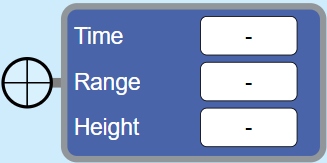
\includegraphics[width=4cm]{physics/figures/phet-projectile-motion.png}}} node[above=1cm]{\texttt[red]{Tool \#1}};
    \end{tikzpicture}
    \hspace{5mm}
    \begin{tikzpicture}
        \begin{scope}
            \clip (0,-0.03) circle (0.87);
            \draw (0,0) node {\fbox{
\includegraphics[width=2cm]{physics/figures/phet-projectile-motion-3.png}}};
            \draw[thick] (0,-0.03) circle (0.85);
        \end{scope}
        \node[above=8mm] at (0,0) {\texttt[red]{Reset button}};
    \end{tikzpicture}
\end{center}

The \texttt[red]{Tool \#1} measures time, range, and height at several points on the path of a projectile. \texttt[red]{Time} is the time elapsed since the launch of the projectile, \texttt[red]{Range} is the projectile's horizontal displacement from the origin, and \texttt[red]{Height} is the projectile's vertical displacement from the origin. Three special points on the trajectory are worth mentioning. First, the origin, which is where the cannon is positioned, defines the initial horizontal and vertical positions of the projectile as zero: $x_0=0$ and $y_0 = 0$. Second, the maximum height occurs when the reaches its largest vertical displacement, and, third, maximum range occurs when the projectile impacts the ground. 

\begin{center}
    \begin{tikzpicture}[
        declare function={f(\x,\yi,\vi,\thetai)=\yi + tan(\thetai)*\x - \grav*\x^2/(2*(\vi*cos(\thetai))^2);}, %equation of path
        declare function={R(\vi,\thetai) = \vi^2 * sin(2*\thetai) / \grav;}, % maximum range
        declare function={h(\vi,\thetai) = (\vi*sin(\thetai))^2/(2*\grav);} %maximum height
    ]
    \tikzmath{
        \grav=9.8;
    }
    \pgfplotsset{compat=1.11}
        \begin{axis}[width=7cm,height=7cm,ticks=none,
        axis lines = center,
        axis line style={draw=none},
        clip=false,
        xmin=0, xmax={R(18,80)*1.1},
        ymin=0, ymax={h(18,80)*1.1},
        ]
        \draw[thick,blue,domain=0:{R(18,80)},variable=\x,samples=200] plot ({\x},{f(\x,0,18,80)});
        \node[left] at (0,0) {origin};
        \node[rotate=72,blue] at (2,7) {trajectory};
        \draw (0.6,0) arc (0:35:2) node[pos=0.8,right=2pt] {\ang{80}};
        \draw[<->,dashed] (0,0) -- ++(axis direction cs: {R(18,80)},0) node[pos=0.8,below] {maximum range};
        \draw[<->,dashed] ({R(18,80)/2},0) -- ++(axis direction cs: 0,{h(18,80)}) node[above] {maximum height};
        \end{axis}
    \end{tikzpicture}
\end{center}

\vspace{1em}

\textbf{Part I: Measuring Time, Range, and Height}

\begin{enumerate}
    \item Click the \texttt[red]{Fire} button to launch a cannonball from the cannon. Observe that the path of the projectile is indicated by the blue curve. A projectile's path is called the trajectory.
    \item Draw a sketch of the trajectory. 
    \item \label{VSHLLm} Use \texttt[red]{Tool \#1} to measure time, range, and height data throughout the trajectory at 0.4-second time intervals. In other words, at times $t=\SI{0.0}{s}$, \SI{0.4}{s}, \SI{0.8}{s}, \ldots, \SI{3.6}{s}. Label your data on the sketch from Step \ref{VSHLLm}.
    \item Record time, range, and height at these three points: the origin, at maximum height, and at maximum range.
\end{enumerate}



\vspace{1em}

\textbf{Part II: How Mass Affects Projectile Path}

\begin{enumerate}
    \item The \texttt[red]{Reset} button ($\boldsymbol{\circlearrowleft}$) is located at the bottom right corner. It resets all settings to the default, as you found the page when you first opened it. Click the $\boldsymbol{\circlearrowleft}$ button.
    \item Click the \texttt[red]{Fire} button to launch a cannonball. Observe the same path, or the so-called trajectory, as before.
    \item \label{thVv3G} The default mass of the cannonball is \SI{17.60}{kg}. Change the mass to \SI{3.00}{kg}, and fire the cannon again. Did the trajectory change? Record your observations. 
    \item Repeat Step \ref{thVv3G} using the following projectile masses: $m=\SI{10}{kg}$, \SI{25}{kg}, and \SI{31}{kg}. Record your observations for each case. Then answer the following question: How does changing the mass of a projectile affect its path?
\end{enumerate}

\vspace{1em}

\textbf{Part III: How Launch Height Affects Projectile Path}
\begin{enumerate}
    \item Click the \texttt[red]{Reset} ($\boldsymbol{\circlearrowleft}$) button.
    \item Click the \texttt[red]{Fire} button, noting the familiar trajectory in blue.
    \item Locate the cannon, at the origin. The values \SI{0}{m} and \ang{80} next to the cannon indicate that the projectile is set to be launched from a height of zero meters and at angle of \ang{80} from the horizontal.
    \item Locate the $\boldsymbol{+}$ symbol on the center of the cannon. Clicking and dragging this symbol upwards increases the launch height of the projectile. Change the launch height to 3 meters, fire the projectile at this height, and observe the new projectile path. Record your observations.
    \item Click-and-drag the $\boldsymbol{+}$ to change the launch height from 0 to 15 meters in increments of 3. In other words, from launch heights of \SI{0}{m}, \SI{3}{m}, \SI{6}{m}, \ldots, \SI{15}{m}. At each launch height, \texttt[red]{Fire} the projectile to observe the new trajectory. Record all your observations. 
    \item How does changing the launch height affect the path of a projectile? You may draw several sketches and use time, range, and height data from \texttt[red]{Tool \#1} to support your answer.
\end{enumerate}

\vspace{1em}

\textbf{Part IV: How Launch Velocity Changes Projectile Path}

\begin{enumerate}
    \item Click $\boldsymbol{\circlearrowleft}$ to reset all settings.
    \item \texttt[red]{Fire} the projectile at the default settings and observe the now-familiar trajectory. 
    \item By default, the cannon is set to fire the projectile with an initial speed (or velocity) of 18 meters per second. Decrease the velocity to \SI{12}{m/s}, \texttt[red]{Fire} the projectile, and observe the new projectile path.
    \item Increase the speed to \SI{24}{m/s}, \texttt[red]{Fire} the projectile, and observe the new trajectory.
    \item What initial speed causes the projectile to land closest to the bullseye (all other factors being equal)?
    \item How does changing launch velocity affect the path of a projectile? Draw sketches and reference time, range, and height data from \texttt[red]{Tool \#1} to support your answer.
\end{enumerate}

\subsection{Projectile Motion} \label{tMF7JY}

\Gls{projectile motion} is the motion of an object thrown (projected) into the air when, after the initial force that launches the object, air resistance is negligible and the only other force that object experiences is the force of gravity. The object is called a \gls{projectile}, and its path is called its \gls{trajectory}. \Gls{air resistance} is a frictional force that slows its motion and can significantly alter the trajectory of the motion. Due to the difficulty in calculation, only situations in which the deviation from projectile motion is negligible and air resistance can be ignored are considered in introductory physics. That approximation is often quite accurate.

\vspace{1em}

The most important concept in projectile motion is that when air resistance is ignored, horizontal and vertical motions are independent, meaning that they don't influence one another. Figure ?.?? compares a cannonball in free fall (in blue) to a cannonball launched horizontally in projectile motion (in red). You can see that the cannonball in free fall falls at the same rate as the cannonball in projectile motion. Keep in mind that if the cannon launched the ball with any vertical component to the velocity, the vertical displacements would not line up perfectly.

\vspace{1em}

Since vertical and horizontal motions are independent, we can analyze them separately, along perpendicular axes. To do this, we separate projectile motion into the two components of its motion, one along the horizontal axis and the other along the vertical.

\begin{center}
    \begin{tikzpicture} 
    \tikzmath{
        \vi = 28.6;
        \yi = 60;
        \thetai = 0.0;
    }
    \tikzset{declare function={f(\x)=\yi + tan(\thetai)*\x - 9.8*\x^2/(2*(\vi*cos(\thetai))^2);}} %equation of path
    \pgfplotsset{compat=1.11}
        \begin{axis}[width=8cm,height=8cm,ticks=none,
        axis lines = center,
        clip=false,
        ylabel = $y$,
        xlabel = $x$,
        xmin=0, xmax=120,
        ymin=0, ymax=80,
        ]
        \draw[dashed,domain=0:100,variable=\x,samples=200] plot ({\x},{f(\x)});
        \draw[dashed] (0,{f(0)}) -- ++(100,0);
        \draw[dashed] (0,{f(0)}) -- ++(0,-{f(0)});
        
        \fill (0,{f(0)}) circle (2pt);
        \fill (20,{f(20)}) circle (2pt); 
        \fill (40,{f(40)}) circle (2pt); 
        \fill (60,{f(60)}) circle (2pt); 
        \fill (80,{f(80)}) circle (2pt); 
        \fill (100,{f(100)}) circle (2pt); 
        
        \draw[dashed] (20,{f(0)}) -- ++(0,{-(f(0)-f(20))});
        \draw[dashed] (40,{f(0)}) -- ++(0,{-(f(0)-f(40))});
        \draw[dashed] (60,{f(0)}) -- ++(0,{-(f(0)-f(60))});
        \draw[dashed] (80,{f(0)}) -- ++(0,{-(f(0)-f(80))});
        \draw[dashed] (100,{f(0)}) -- ++(0,{-(f(0)-f(100))});
        \fill[cyan] (20,{f(0)}) circle (2pt);
        \fill[cyan] (40,{f(0)}) circle (2pt);
        \fill[cyan] (60,{f(0)}) circle (2pt);
        \fill[cyan] (80,{f(0)}) circle (2pt);
        \fill[cyan] (100,{f(0)}) circle (2pt);
        
        \draw[dashed] (0,{f(20)}) -- ++(20,0);
        \draw[dashed] (0,{f(40)}) -- ++(40,0);
        \draw[dashed] (0,{f(60)}) -- ++(60,0);
        \draw[dashed] (0,{f(80)}) -- ++(80,0);
        \draw[dashed] (0,{f(100)}) -- ++(100,0);
        \fill[red] (0,{f(20)}) circle (2pt);
        \fill[red] (0,{f(40)}) circle (2pt);
        \fill[red] (0,{f(60)}) circle (2pt);
        \fill[red] (0,{f(80)}) circle (2pt);
        \fill[red] (0,{f(100)}) circle (2pt);
        \end{axis}
    \end{tikzpicture}
    \captionsetup{type=figure,margin=1in,font=scriptsize}
    \captionof{figure}{The diagram shows the projectile motion of a cannonball shot at a horizontal angle versus one dropped with no horizontal velocity. Note that both cannonballs have the same vertical position over time.}
\end{center}

\vspace{1em}

We'll call the horizontal axis the $x$-axis and the vertical axis the $y$-axis. For notation, $d$ is the total displacement, and $x$ and $y$ are its components along the horizontal and vertical axes. The magnitudes of these vectors are $x$ and $y$, as illustrated in Figure \ref{i1Y7vV}.

\begin{center}
    \begin{tikzpicture} 
    \tikzmath{
        \vi = 18.0;
        \yi = 0;
        \thetai = 70.0;
    }
    \tikzset{declare function={f(\x)=\yi + tan(\thetai)*\x - 9.8*\x^2/(2*(\vi*cos(\thetai))^2);}} %equation of path
    \pgfplotsset{compat=1.11}
        \begin{axis}[width=8cm,height=8cm,ticks=none,
        axis lines = center,
        clip=false,
        ylabel = $y$,
        xlabel = $x$,
        xmin=0, xmax=20,
        ymin=0, ymax=18,
        ]
        \node at (15.6,0.35) {$\square$};
        \draw[dashed,domain=0:16,variable=\x,samples=200] plot ({\x},{f(\x)}) node[above left=-5pt] {\faSoccerBallO};
        \draw[->,thick] (0,0) -- ++(16,{f(16)}) node[pos=0.5,above=3pt]{$d$};
        \draw[->,dashed,thick,cyan] (0,0) -- ++(16,0) node[pos=0.5,below] {$x$};
        \draw[->,dashed,thick,red] (16,0) -- ++(0,{f(16)}) node[pos=0.5,right] {$y$};
        \node at (2.5,0.65) {$\theta$};
        \draw (1.5,0) arc (0:35:1.5);
        \end{axis}
    \end{tikzpicture}
    \captionsetup{type=figure,margin=1in,font=scriptsize}
    \captionof{figure}{A boy kicks a ball at angle $\theta$, and it is displaced a distance of $d$ along its trajectory.}
    \label{i1Y7vV}
\end{center}

\vspace{1em}

As usual, we use velocity, acceleration, and displacement to describe motion. We must also find the components of these variables along the $x$- and $y$-axes. The components of acceleration are then very simple: $a_y = -g = -\SI{9.80}{m/s^2}$. Note that this definition defines the upwards direction as positive. Because gravity is vertical, $a_x = 0$. Both accelerations are constant, so we can use the kinematic equations. For review, the kinematic equations from a previous chapter are summarized below.

\begin{align}
    x &= x_0 + v_{\text{avg}} t\\[0.5ex]
    v_{\text{avg}} &= \frac{v_0 + v}{2}\\[0.5ex]
    v &= v_0 + a t\\[0.5ex]
    x &= x_0 + v_0 t + \frac{1}{2} a t^2\\[0.5ex]
    v^2 &= v_0^2 + 2 a (x - x_0)
\end{align}

where $x$ is position, $x_0$ is initial position, $v$ is velocity, $v_avg$ is average velocity, $t$ is time, and $a$ is acceleration.

\vspace{1em}


  .

\begin{center}
    \begin{tikzpicture}[
        declare function={f(\x)=\yi + tan(\thetai)*\x - 10*\x^2/(2*(\vi*cos(\thetai))^2);},
        declare function={t(\x)=\x/(\vi*cos(\thetai));}
    ]
    \tikzmath{
        \grav = 10;
        \vi = 20;
        \yi = 0;
        \thetai = 45.0;
        \viy = \vi*sin(\thetai);
        \ymax = (\viy^2)/(2*\grav);
        \tmax = 2*\ymax/\viy;
        \vix = \vi*cos(\thetai);
        \xmax = \vix*\tmax;
        \sf = 0.3; %scale factor for vector components
    }
    \pgfplotsset{compat=1.11}
        \begin{axis}[width=12cm,height=12cm,ticks=none,
        axis lines = center,
        clip=false,
        ylabel = $y$,
        xlabel = $x$,
        xmin=0, xmax=50,
        ymin=0, ymax=15,
        ]
        
        \draw[fill=black] (0,0) circle (2pt);
        \draw[thick,violet,->] (0,0) -- ++(\vix*\sf,\viy*\sf) node[below right] {$v_0$};
        \draw[thick,dashed,red,->] (0,0) -- ++(0,{\sf*\vi*sin(\thetai)}) node[right=-2pt] {$v_{0y}$};
        \draw[thick,dashed,cyan,->] (0,0) -- ++(\vix*\sf,0) node[pos=1.3, above=-2pt] {$v_{0x}$};
        \draw (1,0) arc (0:75:0.6) node[midway,right=-1pt] {$\theta_0$};
        
        \pgfplotsinvokeforeach{5,10,15}{
                \draw[fill=black] (#1,{f(#1)}) circle (2pt);
                \draw[thick,dashed,red,->] (#1,{f(#1)}) -- ++(0,{\sf*(\vi*sin(\thetai) - \grav*t(#1))}) node[above=-2pt] {$v_y$};
                \draw[thick,dashed,cyan,->] (#1,{f(#1)}) -- ++(\vix*\sf,0) node[right=-2pt] {$v_x$};
                \draw[thick,violet,->] (#1,{f(#1)}) -- ++(\vix*\sf,{\sf*(\vi*sin(\thetai) - \grav*t(#1))}) node[above=-2pt] {$v$};
                }
                
        \draw[fill=black] (\xmax,\ymax) circle (2pt);
        \draw[thick,violet,->] (\xmax,\ymax) -- ++(\vix*\sf,0) node[right=-2pt] {$v = v_x$};
        
        \pgfplotsinvokeforeach{25,30,35,45}{
                \draw[fill=black] (#1,{f(#1)}) circle (2pt);
                \draw[thick,dashed,red,->] (#1,{f(#1)}) -- ++(0,{\sf*(\vi*sin(\thetai) - \grav*t(#1))}) node[below=-2pt] {$v_y$};
                \draw[thick,dashed,cyan,->] (#1,{f(#1)}) -- ++(\vix*\sf,0) node[right=-2pt] {$v_x$};
                \draw[thick,violet,->] (#1,{f(#1)}) -- ++(\vix*\sf,{\sf*(\vi*sin(\thetai) - \grav*t(#1))}) node[below=-2pt] {$v$};
                }

                \draw[fill=black] (40,{f(40)}) circle (2pt);
                \draw[thick,dashed,red,->] (40,{f(40)}) -- ++(0,{\sf*(\vi*sin(\thetai) - \grav*t(40))}) node[left=-2pt] {$v_y=-v_{0y}$};
                \draw[thick,dashed,cyan,->] (40,{f(40)}) -- ++(\vix*\sf,0) node[above=-2pt] {$v_x$};
                \draw[thick,violet,->] (40,{f(40)}) -- ++(\vix*\sf,{\sf*(\vi*sin(\thetai) - \grav*t(40))}) node[below=-2pt] {$v$};
                \draw (40.8,0) arc (0:-\thetai:0.8) node[midway,right=-1pt] {$\theta =-\theta_0$};

                \draw (5.8,{f(5)}) arc (0:40:0.8) node[midway,right] {$\theta$};
        \end{axis}
    \end{tikzpicture}
    \captionsetup{type=figure,font=scriptsize}
    \captionof{figure}{We analyze two-dimensional projectile motion by breaking it into two independent one-dimensional motions along the vertical and horizontal axes. The horizontal motion is constant. The velocity in the vertical direction begins to decrease, then becomes zero at the peak, then increases in the downward direction.}
    \label{xRbMxN}
\end{center}

\clearpage

\begin{exercise}
    If an object is thrown horizontally, travels with an average x-component of its velocity equal to \SI{5}{m/s}, and does not hit the ground, what will be the $x$-component of the displacement after \SI{20}{s}? 

    \begin{enumerate}[label=\Alph*.]
        \item \SI{-100}{m}
        \item \SI{-4}{m}
        \item \SI{4}{m}
        \item \SI{100}{m}
    \end{enumerate}
\end{exercise}

\begin{exercise}
    If a ball is thrown straight up with an initial velocity of \SI{20}{m/s} upward, what is the maximum height it will reach?

    \begin{enumerate}[label=\Alph*.]
        \item \SI{-20.4}{m}
        \item \SI{-1.02}{m}
        \item \SI{1.02}{m}
        \item \SI{20.4}{m}
    \end{enumerate}
\end{exercise}






The fact that vertical and horizontal motions are independent of each other lets us predict the range of a projectile. The \gls{range} is the horizontal distance $R$ traveled by a projectile on level ground, as illustrated in Figure \ref{6hKQ2Y}. Throughout history, people have been interested in finding the range of projectiles for practical purposes, such as aiming cannons.

\begin{center}
    \begin{tikzpicture}[
        declare function={f(\x,\yi,\vi,\thetai)=\yi + tan(\thetai)*\x - \grav*\x^2/(2*(\vi*cos(\thetai))^2);}, %equation of path
        declare function ={R(\vi,\thetai)= \vi^2*sin(2*\thetai)/\grav;}, %range
        declare function={h(\vi,\thetai)=(\vi*sin(\thetai))^2/(2*\grav);}, %maximum height
    ]
    \tikzmath{
        \grav = 9.8;
        \sf = 0.5; %scale factor for vector components
    }
    \pgfplotsset{compat=1.11}
        \begin{axis}[width=12cm,height=5cm,ticks=none,
        axis lines = center,
        clip=false,
        ylabel = $y$,
        xlabel = $x$,
        xmin=0, xmax={R(50,45)*1.1},
        ymin=0, ymax={h(50,45)*1.1},
        ]
        \draw[Green,thick,->] (0,0) -- ++({50*cos(45)},{50*sin(45)}) node[above left=-5pt] {\SI{50}{m/s}};;
        \draw[Green,thick,domain=0:{R(50,45)},variable=\x,samples=250] plot ({\x},{f(\x,0,50,45)}) node[black,below] {$R = \SI{225}{m}$};
        \draw[violet,thick,->] (0,0) -- ++({40*cos(45)},{40*sin(45)}) node[pos=0.93,right=2.7mm] {\SI{40}{m/s}};;
        \draw[violet,thick,domain=0:{R(40,45)},variable=\x,samples=250] plot ({\x},{f(\x,0,40,45)}) node[black,below] {$R = \SI{163}{m}$};
        \draw[red,thick,->] (0,0) -- ++({30*cos(45)},{30*sin(45)}) node[pos=0.4,right=3pt] {\SI{30}{m/s}, \ang{45}};
        \draw[red,thick,domain=0:{R(30,45)},variable=\x,samples=250] plot ({\x},{f(\x,0,30,45)})
    node[black,below] {$R = \SI{91.8}{m}$};;
        \end{axis}
    \end{tikzpicture}

    \vspace{1em}

    \begin{tikzpicture}[
        declare function={f(\x,\yi,\vi,\thetai)=\yi + tan(\thetai)*\x - \grav*\x^2/(2*(\vi*cos(\thetai))^2);}, %equation of path
        declare function ={R(\vi,\thetai)= \vi^2*sin(2*\thetai)/\grav;}, %range
        declare function={h(\vi,\thetai)=(\vi*sin(\thetai))^2/(2*\grav);}, %maximum height
    ]
    \tikzmath{
        \grav = 9.8;
        \sf = 0.5; %scale factor for vector components
    }
    \pgfplotsset{compat=1.11}
        \begin{axis}[width=12cm,height=5cm,ticks=none,
        axis lines = center,
        clip=false,
        ylabel = $y$,
        xlabel = $x$,
        xmin=0, xmax={R(50,45)*1.1},
        ymin=0, ymax={h(50,75)*1.1},
        ]
        \draw[Green,thick,->] (0,0) -- ++({50*cos(75)},{50*sin(75)}) node[pos=1.7,rotate=58] {\SI{50}{m/s}, \ang{75}};;
        \draw[Green,thick,domain=0:{R(50,75)},variable=\x,samples=250] plot ({\x},{f(\x,0,50,75)}) node[black,below] {$R = \SI{128}{m}$};
        \draw[violet,thick,->] (0,0) -- ++({50*cos(45)},{50*sin(45)}) node[pos=1.6,rotate=20,below=-6pt] {\SI{50}{m/s}, \ang{45}};;
        \draw[violet,thick,domain=0:{R(50,45)},variable=\x,samples=250] plot ({\x},{f(\x,0,50,45)}) node[black,below] {$R = \SI{225}{m}$};
        \draw[red,thick,->] (0,0) -- ++({50*cos(15)},{50*sin(15)}) node[pos=1.5] {\SI{50}{m/s}, \ang{15}};;
        \draw[red,thick,domain=0:{R(50,15)},variable=\x,samples=250] plot ({\x},{f(\x,0,50,15)});
        \end{axis}
    \end{tikzpicture}
    \captionsetup{type=figure,margin=1in,font=scriptsize}
    \captionof{figure}{Trajectories of projectiles on level ground. \textit{Top plot}: The greater the initial speed,$v_0$, the greater the range for a given initial angle. \textit{Bottom plot}: The effect of initial angle, $\theta_0$, on the range of a projectile with a given initial speed. Note that any combination of trajectories that add to 90 degrees will have the same range in the absence of air resistance, although the maximum heights of those paths are different.}
    \label{6hKQ2Y}
\end{center}

How does the initial velocity of a projectile affect its range? Obviously, the greater the initial speed $v_0$, the greater the range, as shown in the figure above. The initial angle $\theta_0$ also has a dramatic effect on the range. When air resistance is negligible, the range $R$ of a projectile on level ground is

\begin{equation} \label{GqvaN1}
    R = \frac{v_0^2 \sin{(2\theta_0)}}{g}
\end{equation}

where $v_0$ is the initial speed and $\theta_0$ is the initial angle relative to the horizontal. It is important to note that the range doesn't apply to problems where the initial and final $y$ position are different, or to cases where the object is launched perfectly horizontally.

\begin{exercise}
    What is projectile motion?
    
    \begin{enumerate}[label=\Alph*.]
        \item Projectile motion is the motion of an object projected into the air and moving under the influence of gravity.
        \item Projectile motion is the motion of an object projected into the air and moving independently of gravity.
        \item Projectile motion is the motion of an object projected vertically upward into the air and moving under the influence of gravity.
        \item Projectile motion is the motion of an object projected horizontally into the air and moving independently of gravity.
    \end{enumerate}
\end{exercise}

\begin{exercise}
    What is the force experienced by a projectile after the initial force that launched it into the air in the absence of air resistance?

    \begin{enumerate}[label=\Alph*.]
        \item The nuclear force
        \item The gravitational force
        \item The electromagnetic force
        \item The contact force
    \end{enumerate}
\end{exercise}






\subsection{Uniform Circular Motion} \label{uPOucv}

Circular motion is when an object moves in a circular path. Examples of circular motion include a race car speeding around a circular curve, a toy attached to a string swinging in a circle around your head, or the circular loop-the-loop on a roller coaster. The simplest case of circular motion is \gls{uniform circular motion}, where an object travels a circular path at a constant speed. Note that, unlike speed, the linear velocity of an object in circular motion is constantly changing because it is always changing direction. We know that acceleration is a change in velocity, either in magnitude or in direction or both. Therefore, an object undergoing uniform circular motion is always accelerating, even though the magnitude of its velocity is constant.

\vspace{1em}

You experience this acceleration yourself every time you ride in a car while it turns a corner. If you hold the steering wheel steady during the turn and move at a constant speed, you are executing uniform circular motion. What you notice is a feeling of sliding (or being flung, depending on the speed) away from the center of the turn. This isn't an actual force that is acting on you---it only happens because your body wants to continue moving in a straight line (as per Newton's first law) whereas the car is turning off this straight-line path. Inside the car it appears as if you are forced away from the center of the turn. This fictitious force is known as the \gls{centrifugal force}. The sharper the curve and the greater your speed, the more noticeable this effect becomes.

\begin{center}
\begin{tikzpicture}
    \begin{axis}[
        width=7cm,height=7cm,
        axis line style={draw=none},
        ticks=none,
        axis lines=middle,
        xmin=-1,xmax=1,
        ymin=-1,ymax=1,
        clip=false,
    ]
    \draw[gray] (0,0) circle (1);
    \fill (0,0) circle (1pt);
    \fill ({cos(45)},{sin(45)}) circle (3pt) node[above right] {$m$};
    \begin{scope}[shift={(axis direction cs: 0.04,-0.04)}]
        \draw[dashed,<->] (0,0) -- ({cos(45)},{sin(45)}) node[pos=0.5,below right=-1pt] {$r$};
    \end{scope}
    \draw[Green,very thick,->] ({cos(45)},{sin(45)}) -- ++(axis direction cs: -0.3,-0.3) node[black,above=5pt,pos=1.2] {$a_{\text{c}}$};
    \draw[red,very thick,->] ({cos(45)},{sin(45)}) -- ++(axis direction cs: -0.6,0.6) node[black,pos=1.1] {$v$};
\end{axis}
\end{tikzpicture}
\captionsetup{type=figure,margin=1in,font=scriptsize}
\captionof{figure}{Uniform circular motion, the radius of curvature and vectors for tangential velocity and centripetal acceleration. Compare this with the Ladybug Motion Simulation in Exercise \ref{N066SF}.}
\label{4QmpMJ}
\end{center}

Other examples of (approximate) uniform circular motion include the \href{https://youtu.be/3NYlYN-QTig}{hammer throw}, a bicyclist rounding a turn on a curved path, and the Earth's orbit around the Sun. The \gls{tangential velocity} ($\vec{v}$) is the instantaneous linear velocity of the object in circular motion. If the circular motion is abruptly cut off (as in the hammer throw sport), the object moves in a straight line in the direction of the tangential velocity. \Gls{tangential speed} is the magnitude of the tangential velocity, with no regard for the direction. The \gls{radius of curvature} ($r$) is the distance between the center of the circle and the path. We call the acceleration of an object moving in uniform circular motion the \gls{centripetal acceleration} ($a_c$) because centripetal means \textit{center seeking}.

\vspace{1em}

Now that we know that the direction of centripetal acceleration is toward the center of rotation, let's discuss the magnitude of centripetal acceleration. For an object traveling at speed $v$ in a circular path with radius $r$, the magnitude of centripetal acceleration is


\begin{equation} \label{5vsZ8y}
    a_{\text{c}} = \frac{v^2}{r}\ 
\end{equation}

\begin{center}
    \begin{tabular}{cl|cl}
    \hline
    \textbf{Symbol} & \textbf{Quantity} & \textbf{Unit} & \textbf{Unit Symbol}  \\
    \hline\hline
    \rule{0pt}{2.5ex}
        $a_{\text{c}}$ & centripetal acceleration & meter per second squared & \SI{}{m/s^2}\\
        $v$ & tangential speed & meter per second & \SI{}{m/s} \\
        $r$ & radius & meter & \SI{}{m}\\
    \hline
    \end{tabular}
\end{center}

Centripetal acceleration is greater at high speeds and in sharp curves (smaller radius), as you may have noticed when driving a car, because the car actually pushes you toward the center of the turn. But it is a bit surprising that ac is proportional to the speed squared. This means, for example, that the acceleration is four times greater when you take a curve at \SI{20}{m/s} than at \SI{10}{m/s}.

\vspace{1em}

Because an object in uniform circular motion undergoes acceleration (by changing the direction of motion but not the speed), we know from Newton's second law of motion that there must be a net external force acting on the object. Since the magnitude of the acceleration is constant, so is the magnitude of the net force, and since the acceleration points toward the center of the rotation, so does the net force.

\vspace{1em}

Any force or combination of forces can cause a centripetal acceleration. Just a few examples are the tension in the rope on a tether ball, the force of Earth's gravity on the Moon, the friction between a road and the tires of a car as it goes around a curve, or the normal force of a roller coaster track on the cart during a loop-the-loop.

\vspace{1em}

The component of any net force that causes circular motion is called a \gls{centripetal force}. When the net force is equal to the centripetal force, and its magnitude is constant, uniform circular motion results. The direction of a centripetal force is toward the center of rotation, the same as for centripetal acceleration. According to Newton's second law of motion, a net force causes the acceleration of mass according to 

\begin{equation*}
    F_{\text{net}} = ma
\end{equation*}

For uniform circular motion, the acceleration is centripetal acceleration: 

\begin{equation*}
    a = a_c
\end{equation*}

Therefore, the magnitude of centripetal force, $F_c$, is $F_c = m a_c$. By using Equation \eqref{5vsZ8y} for the magnitude of centripetal acceleration, $a_c = v^2/r$, we get an expression involving the magnitude of the centripetal force in terms of tangential speed:

\begin{equation} \label{4H9EJq}
    F_c = m a_c = \frac{m v^2}{r}
\end{equation}

\begin{center}
    \begin{tabular}{cl|cl}
    \hline
    \textbf{Symbol} & \textbf{Quantity} & \textbf{Unit} & \textbf{Unit Symbol}  \\
    \hline\hline
    \rule{0pt}{2.5ex}
        $F_{\text{c}}$ & centripetal force & newton & N\\
        $m$ & mass & kilogram & \SI{}{kg}\\
        $v$ & tangential speed & meter per second & \SI{}{m/s} \\
        $r$ & radius & meter & \SI{}{m}\\
    \hline
    \end{tabular}
\end{center}

Newton's second law also states that the object will accelerate in the same direction as the net force. By definition, the centripetal force is directed towards the center of rotation, so the object will also accelerate towards the center. A straight line drawn from the circular path to the center of the circle will always be perpendicular to the tangential velocity. 

\begin{example}
    A car follows a curve of radius \SI{500}{m} at a speed of \SI{25.0}{m/s} (about \SI{56}{mph}). What is the magnitude of the car's centripetal acceleration?
\end{example}

\Solution We are given the radius of curvature and the tangential velocity:

\begin{equation*}
    r = \SI{500}{m} \quad \text{and} \quad v = \SI{25}{m/s}
\end{equation*}

The unknown is centripetal acceleration: $a_c =\ ?$. By Equation \eqref{5vsZ8y},

\begin{equation*}
    a_c = \frac{v^2}{r} = \frac{25^2}{500} = 1.25 
\end{equation*}

The centripetal acceleration on the car is \SI{1.25}{m/s} (about 13\% of $g$, the acceleration due to gravity).

\endsolution

\begin{example}
    What is the centripetal force exerted on a \SI{1600}{kg} car that rounds a \SI{100}{m} radius curve at \SI{12}{m/s}?
\end{example}

\Solution We are given mass, radius, and speed:

\begin{equation*}
    m = \SI{1600}{kg}\ , \quad 
    r = \SI{100}{m}\ , \quad
    v = \SI{12}{m/s}
\end{equation*}

The unknown is centripetal force: $F_c =\ ?$ The given and unknown values are related Equation \eqref{4H9EJq}:

\begin{equation*}
    F_c = \frac{m v^2}{r} = \frac{(1600)(12^2)}{100} = 2304
\end{equation*}

The centripetal force is 2304 newtons inward. 

\endsolution

\subsection{Exercises}

\subsubsection*{\nameref{tMF7JY}}

\begin{exercise} \label{90PABl}
    What is the angle between the $x$ and $y$ components of a vector?
\end{exercise}

\begin{exercise}
    Horizontal and vertical motions of a projectile are independent of each other. What does this mean?
\end{exercise}

\begin{exercise} \label{YYBBp5}
    Using the conventional choice for positive and negative axes described in the text, what is the $y$-component of the acceleration of an object experiencing projectile motion?
\end{exercise}

\begin{exercise}  \label{agp59Z}
    Two identical items, object 1 and object 2, are dropped from the top of a \SI{50.0}{m} building. Object 1 is dropped with an initial velocity of \SI{0}{m/s}, while object 2 is thrown straight downward with an initial velocity of \SI{13.0}{m/s}. What is the difference in time, in seconds rounded to the nearest tenth, between when the two objects hit the ground?
\end{exercise}

\begin{exercise} \label{Xu3FK9}
    A water balloon cannon is fired at \SI{30}{m/s} at an angle of \ang{50} above the horizontal. How far away will it fall?
\end{exercise}

\begin{exercise} \label{piJ9kJ}
    A person wants to fire a water balloon cannon such that it hits a target \SI{100}{m} away. If the cannon can only be launched at \ang{45} above the horizontal, what should be the initial speed at which it is launched?
\end{exercise}

\begin{exercise} \label{sy5RGT}
    After a projectile is launched in the air, in which direction does it experience constant, non-zero acceleration, ignoring air resistance?
\end{exercise}

\begin{exercise} \label{N0Bwou}
    A ball is thrown in the air at an angle of \ang{40}. If the maximum height it reaches is \SI{10}{m}, what must be its initial speed?
\end{exercise}

\begin{exercise} \label{lhjg95}
    A large rock is ejected from a volcano with a speed of \SI{30}{m/s} and at an angle \ang{60} above the horizontal. The rock strikes the side of the volcano at an altitude of \SI{10.0}{m} lower than its starting point. Calculate the horizontal displacement of the rock.
\end{exercise}

\begin{exercise} \label{wlbvvu}
    How can you express the velocity, $v$, of a projectile in terms of its initial velocity, $v_0$, acceleration, $g$, and time, $t$?
\end{exercise}

% \begin{exercise}
%     In the equation for the maximum height of a projectile, what does $v_{0y}$ stand for?

% \begin{equation*}
%     h = \frac{v_{0y}^2}{2g}
% \end{equation*}
% \end{exercise}

\begin{exercise} \label{xj6gln}
    True or False? Range is defined as the maximum vertical distance travelled by a projectile. 
\end{exercise}

\begin{exercise} \label{5wfdN0}
    For what angle of a projectile is its range equal to zero?
\end{exercise}

\begin{exercise} \label{DnqDpu}
    Ignoring drag, what is the $x$-component of the acceleration of a projectile? Why?
\end{exercise}

\begin{exercise} \label{QsBUvP}
    What is the optimum angle at which a projectile should be launched in order to cover the maximum distance?
\end{exercise}

\subsubsection*{Uniform Circular Motion}

\begin{exercise} \label{N066SF}
    Bring Figure \ref{4QmpMJ} to life by taking the following steps:

    \begin{enumerate}
        \item Access the OpenStax Simulations (\href{https://veillette.github.io/simulations/}{click here}).
        \item Click the simulation called ``Ladybug Motion.''
        \item Under \texttt[Green]{Vectors}, check the boxes for \texttt[Green]{Show Velocity} and \texttt[Green]{Show Acceleration}. 
        \item Towards the bottom, click \texttt[red]{Velocity}. Then, under \texttt[Green]{Remote Control}, drag the red button until you generate a red arrow about 1 centimeter in length. The Ladybug will start moving.
        \item When the Ladybug is in motion, locate the \texttt[Green]{Motion} options, and select \texttt[Green]{Circular}. The Ladybug is now undergoing uniform circular motion.
        \item Draw a sketch of the Ladybug and its velocity and acceleration vectors. Compare your sketch to Figure \ref{4QmpMJ}. 
    \end{enumerate}
\end{exercise}

\begin{exercise} \label{x2YCzr}
    What is meant by the word \textit{centripetal}?
\end{exercise}

\begin{exercise} \label{S4rGIt}
    (a) What is the direction of the velocity of an object in uniform circular motion? (b) What is the direction of the acceleration?
\end{exercise}

\begin{exercise} \label{aVu3ZA}
    Suppose you have an object tied to a rope and are rotating it over your head in uniform circular motion. If you increase the length of the rope, would you have to apply more or less force to maintain the same speed?
\end{exercise}

\begin{exercise} \label{kTvEZX}
    What is the centripetal acceleration felt by the passengers of a car moving at \SI{12}{m/s} along a curve with radius \SI{2.0}{m}?
\end{exercise}


\begin{exercise} \label{MJm5VE}
    Find the frictional force between the tires and the road that allows a \SI{1000}{kg} car traveling at \SI{30}{m/s} to round a \SI{20}{m} radius curve.
\end{exercise}

\begin{exercise} \label{fsjtBV}
    Which of the following quantities is constant in uniform circular motion? Speed, velocity, acceleration, displacement.
\end{exercise}

\begin{exercise} \label{GD8Yff}
    List the three quantities that influence centripetal force.
\end{exercise}

\begin{exercise} \label{aEtlVz}
    An increase in the magnitude of the \rule{2cm}{0.15mm} causes a \textit{reduction} in the centripetal force.
\end{exercise}

\begin{exercise} \label{5lauZ6}
    What happens to centripetal acceleration as the radius of curvature \textit{decreases} and the speed is held constant? Why?
\end{exercise}

\begin{exercise} \label{KB7t4k}
    Why do we experience more sideways acceleration while driving around sharper curves?
\end{exercise}

\begin{exercise} \label{jb3iGO}
    Is centripetal acceleration a vector or a scalar?
\end{exercise}

\begin{exercise} \label{TUxTQh}
    What are the units of centripetal acceleration?
\end{exercise}

\begin{exercise} \label{9YKhPo}
    What are the units of centripetal force?
\end{exercise}

\begin{exercise} \label{wS6Htw}
    What is the angle formed between the vectors of tangential velocity and centripetal force?
\end{exercise}

\begin{exercise} \label{barV9C}
    What is the angle formed between the vectors of centripetal acceleration and centripetal force?
\end{exercise}

\begin{exercise} \label{M6NkHB}
    As the mass of an object in uniform circular motion increases, what happens to the centripetal force required to keep it moving at the same speed?
\end{exercise}

\begin{exercise} \label{IAjJBC}
    Is an object in uniform circular motion accelerating? Why or why not?
\end{exercise}

\begin{exercise} \label{G8I4Up}
    An object is in uniform circular motion. Suppose the centripetal force was removed. In which direction would the object now travel?
\end{exercise}

\begin{exercise} \label{Kv8Old}
An 89-kg system consisting of a bicycle and rider are rounding a turn at \SI{16}{m/s} on a path with a radius of curvature of \SI{25}{m}. (a) What is the centripetal acceleration on the system? (b) What is the centripetal force?
\end{exercise}


\clearpage


\subsection{Answers to Select Exercises}
\ref{90PABl}. \ang{90}\\
\ref{YYBBp5}. \SI{-9.8}{m/s^2}\\
\ref{agp59Z}. \SI{1.1}{s}\\
\ref{Xu3FK9}. \SI{90.4}{m}\\
\ref{piJ9kJ}. \SI{31.3}{m/s}\\
\ref{sy5RGT}. Vertical (or $y$)\\
\ref{N0Bwou}. \SI{21.8}{m/s}\\
\ref{lhjg95}. \SI{84.9}{m}\\
\ref{wlbvvu}. See Equation \eqref{SjYaoE}\\
\ref{xj6gln}. Range is horizontal.\\
\ref{5wfdN0}. \ang{0} or \ang{90}\\
\ref{DnqDpu}. \SI{0}{m/s^2}. Gravitational acceleration is vertical only.\\
\ref{QsBUvP}. \ang{45}\\
\ref{x2YCzr}. Center-seeking\\
\ref{S4rGIt}. (a) tangential \hspace{1em} (b) radially inward.\\
\ref{aVu3ZA}. Less force. In Equation~(\ref{qzzym8}), radius (the length of the rope) is in the denominator of the fraction. This means that force and radius are \textit{inversely proportional}: if one goes up, the other goes down. By \textit{increasing} the radius (the length of the rope), the centripetal force must \textit{decrease}.
\ref{kTvEZX}. \SI{72}{m/s^2}\\
\ref{MJm5VE}. \SI{45000}{N}\\
\ref{fsjtBV}. Speed. The others are vectors whose directions may change.\\
\ref{GD8Yff}. Mass, speed, and radius. See Eq.~(\ref{qzzym8}).\\
\ref{aEtlVz}. radius of curvature\\
\ref{5lauZ6}. Acceleration is inversely proportional to radius (Eq.~\ref{5vsZ8y}). Therefore, assuming speed stays the same, as radius \textit{decreases} (as the circle gets smaller), acceleration \textit{increases}. See, also, Exercise \ref{aVu3ZA}.\\
\ref{KB7t4k}. Sharper curve means smaller radius of curvature. As radius decreases, acceleration increases. See Exercise \ref{5lauZ6}.\\
\ref{jb3iGO}. vector\\
\ref{TUxTQh}. meters per second squared (\SI{}{m/s^2})\\
\ref{9YKhPo}. newton (N)\\
\ref{wS6Htw}. \SI{90}{\degree}\\
\ref{barV9C}. \SI{0}{\degree}\\
\ref{M6NkHB}. Centripetal force must increase. Equation (\ref{qzzym8}) suggests that force and mass are \textit{directly proportional}: if one increases, the other goes increases too. \\
\ref{IAjJBC}. Yes. Although the object is not speeding up or slowing down, the direction of the velocity vector continuously changes. \\
\ref{G8I4Up}. In the direction of the tangential velocity at the instant the force was removed.\\
\ref{Kv8Old}. (a) \SI{10.24}{m/s^2} \hspace{1em} (b) \SI{911}{N}\\


\end{document}